% Created 2021-12-23 Do 13:35
% Intended LaTeX compiler: pdflatex
\documentclass[ebook]{article}
\usepackage[utf8]{inputenc}
\usepackage[T1]{fontenc}
\usepackage{graphicx}
\usepackage{longtable}
\usepackage{wrapfig}
\usepackage{rotating}
\usepackage[normalem]{ulem}
\usepackage{amsmath}
\usepackage{amssymb}
\usepackage{capt-of}
\usepackage{hyperref}
\usepackage{color}
\usepackage{listings}
\usepackage[english]{babel}
\usepackage[left=2.0cm,right=2.0cm,top=2.5cm,bottom=2.0cm]{geometry}
\makeatother
\usepackage{color}
\definecolor{marron}{RGB}{60,30,10}
\definecolor{darkblue}{RGB}{0,0,80}
\definecolor{lightblue}{RGB}{80,80,80}
\definecolor{darkgreen}{RGB}{0,80,0}
\definecolor{darkgray}{RGB}{0,80,0}
\definecolor{darkred}{RGB}{80,0,0}
\definecolor{shadecolor}{rgb}{0.97,0.97,0.97}
\usepackage{titlesec}
\usepackage{fancyhdr}
\input GoudyIn.fd
\newcommand*\initfamily{\usefont{U}{GoudyIn}{xl}{n}}
\usepackage{lettrine}
\newcommand{\cb}[1]{\lettrine[lines=3]{#1}}
\usepackage{fouriernc}
\usepackage{venturisold}
\newcommand{\sectionbreak}{\clearpage}
\renewcommand\thesection{}
\renewcommand\thesubsection{}
\graphicspath{{figures/}}
\date{}
\title{Simons \\ wunderbare \\ Weihnachtsgeschichte(n)}
\hypersetup{
 pdfauthor={},
 pdftitle={Simons \\ wunderbare \\ Weihnachtsgeschichte(n)},
 pdfkeywords={},
 pdfsubject={},
 pdfcreator={Emacs 29.0.50 (Org mode 9.5.1)}, 
 pdflang={Germanb}}
\begin{document}

\begin{titlepage}
\centering
{\huge Simons \\ wunderbare \\ Weihnachtsgeschichte(n) \par }
\vspace{2cm}
{\large  \par}
\vspace{3cm}
\begin{figure}[h]\hspace*{-0.73cm}\begin{center}
\includegraphics{santa}\end{center}\end{figure}\end{titlepage}

\section{Vorwort}
\label{sec:org6e34148}
Alle Jahre wieder \ldots{}

\noindent Hallo lieber Leser, liebe Leserin, liebes Lesikon. Wenn du
dies ließt, dann wurdest du mit meiner alljährlichen
Weihnachtsgeschichte bedacht. Die Weihnachtsgeschichte begann in
einem Jahr in dem ich entweder zu pleite oder zu faul war Geschenke
zu kaufen. So oder so es führte dazu, dass ich nun schon seit
etlichen Jahren, ein selbst-gebasteltes Geschenk unter die Leute
bringe. Dabei ist wie immer ganz wichtig, das alles, was ich hier
von meinen Fingern per Computer zu Papier bringen selbstverständlich
die Wahrheit und nur die Wahrheit ist. Außerdem sollte beachtet
werden, das der Konsum von bewusstseinserweiternde Substanzen zwar
nicht notwendig für das Lesen dieser Geschichten ist - sich aber
vermutlich durchaus positiv darauf auswirkt. Daher schon mal an
dieser Stelle - nimm dir ein Glas Kinderpunsch mit Schuss oder einen
schönen Weihnachtssekt und gib für einige Minuten vor du würdest
diese Geschichte wirklich lesen. Hahaha und wenn du bis hier her
gekommen bist - irgendwo in der Geschichte die richtigen 6 Lotto
Zahlen versteckt. Und wie jedes Jahr - wer Rechtschreibfehler findet
meldet diese bitte in den Kommentarsection eines Youtubevideos der
AfD, dann steht da auch mal was halbwegs Sinnvolles.

\begin{center}
  Lieber Leser, ich wünsche dir schöne Weihnachten oder ein beliebiges Heidnisches Fest deiner Wahl, das zufällig auf den gleichen Tag fällt. Und natürlich viel Spaß beim Lesen und dann später einen guten Rutsch in neue Jahr.
\end{center}
\section{Frankenstein}
\label{sec:orgd274fd6}
\begin{center}
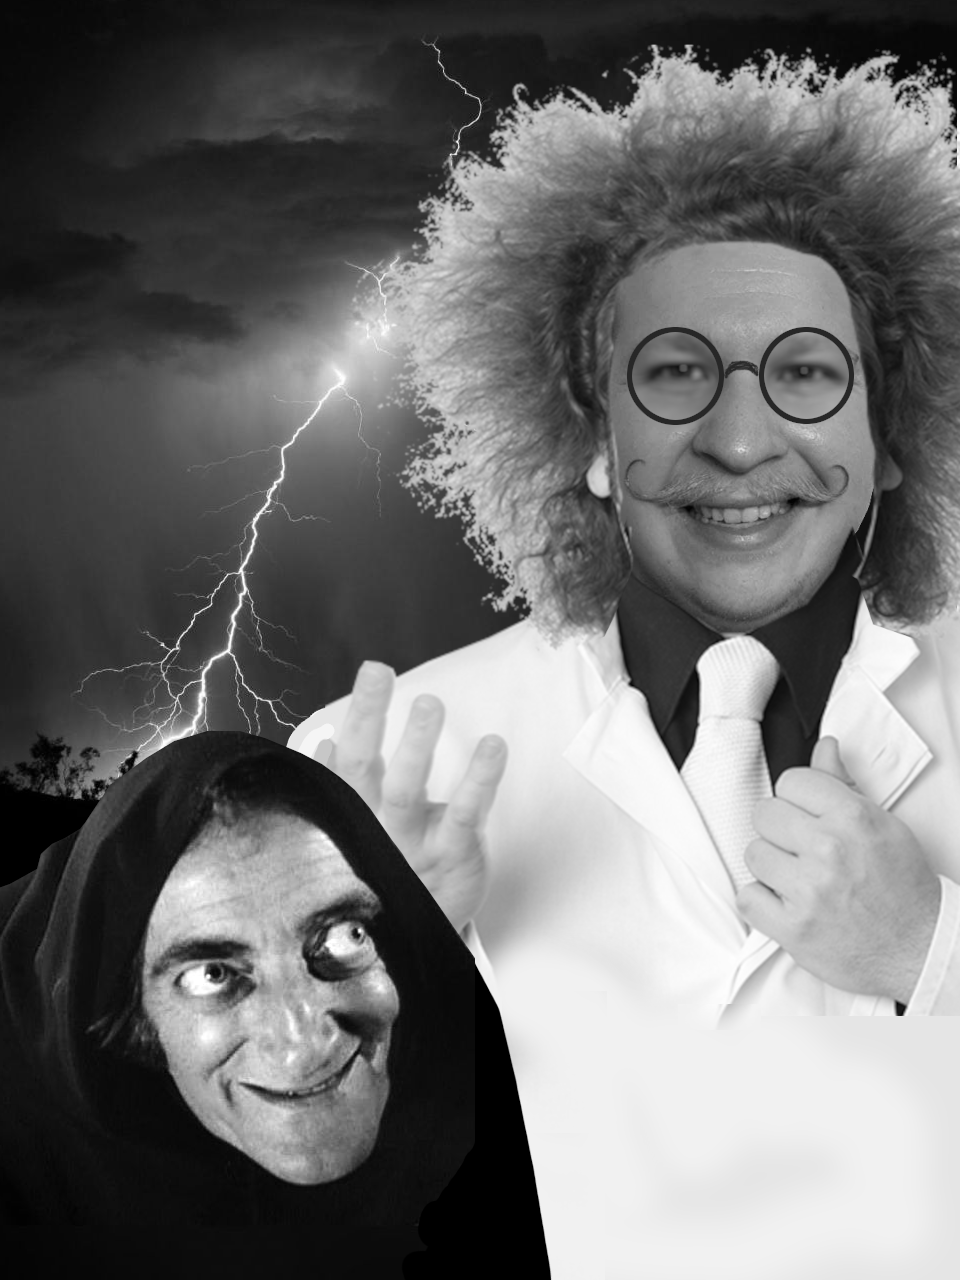
\includegraphics[width=8cm]{frankesteiner.png}
\end{center} \cb{D}ie Peitsche knallte im
transsilvanischen Mondschein. Ein Wolfs-heulen in der Ferne
übertönte das Rattern der Kutsche. Es war arschkalt. Nein wirklich!
Der Wind rüttelte an den eisbeschlagenen Fenstern, die bei jedem
Stein beunruhigend knackende Geräusche machten. Mein Atem bildete
Nebelschwaden vor meinem Gesicht. Ich schlang meine Arme enger um
mich. Mir gegenüber saß eine alte Frau - über und über in bunte
Stoff gehüllt, die unbeirrt Gebete murmelte, sich bekreuzigte und
abwechselnd mit einer Weihwasser Kelle nach mir spritzte und
abfällig vor meine Füße spukte. Genervt versuchte ich mich auf etwas
anderes als den Aberglauben dieser netten Dame zu konzentrieren -
z.B. das bedrohlich näher kommende Wolfsgeheul gerade als Madame in
ihrem Mantra mal wieder dabei war gurgelnd Spucke in ihrem Schlund
zu sammeln ertönte ein Ruf des Kutschers, gefolgt von einem
Quietschen. Zeitversetzt kam die Spuckerin in meine Richtung
geflogen! Ich konnte gerade noch ausweichen; Sie knallte mit
Schmackes links neben mir auf die Sitzbank und das Gefährt war zum
Stehen gekommen. Der Kutscher sprang dumpf in den Schnee, watschelte
um die Kutsche und öffnete die Tür. Noch kältere Luft drang ins
Innere. Der Kutscher hielt seinen Arm ins innere, die nun
verdatterte Dame griff danach. Ohne lange zu fackeln zog der Mann
den Arm samt Frau aus der Kutsche und stellte sie hin. Durch die Tür
sah ich eine Reihe von Menschen in einer mir unbekannten Tracht. Die
Tür schwang zu. Kurz darauf fuhr die Kutsche wieder an. Nun war ich
zwar verschont davon gleichzeitig gesegnet und oder exorziert zu
werden, aber dafür war mir jetzt langweilig.

\noindent Ich beschloss den Brief nochmal zu lesen, der die Ursache
für meine Reise war. Dieser komische Brief. Vor ein paar Wochen
hatte ich mal wieder meinen Briefkasten ausgeleert und zwischen
Werbung und Werbung und noch mehr Werbung befand sich ein
ungewöhnlicher Brief. Der Versender hatte das beschriebene Blatt,
ein grobes, gelbliches Papier, so gefaltet das ein Brief daraus
wurde. Um den \emph{Umschlag} zu schließen prankte er schweres rotes
Wachssiegel mit einem mittelalterlichen Wappen der Frontseite. Die
Nachricht im Inneren, war jedoch noch ungewöhnlicher!

\noindent Der Kutscher knallte seine Peitsche, es Quietschte und
Augenblicke vor dem Aufprall erinnerte ich mich daran das ich beim
letzten Halt auf den warmen Platz der Spuckerin gewechselt war. Der
Schmerz in meinen Gliedern übertönte die Kälte. Die Tür sprang auf,
ein Arm schnellte herein und packte mich. Sanfter als erwartet
stellte der Kutscher mich ab. Er tippte sich an die Hutkrempe,
nickte mir aufmunternd zu und watschelte Richtung Kutschbock. Wir
waren an unserem Ziel angekommen. Ich hob meinen Blick und starrte
fassungslos die massiven Mauern, die Zugbrücke, Türme und Mauern
an. Es hatte aufgehört zu schneien, so als hätte das heimliche,
flauschige Weich Angst sich auf den Dächern der bedrohlichen Burg
nieder zu lassen. Während die Kutsche sich schlingernd entfernte
erschien eine ominöse Gestalt auf der Zugbrücke. Ein kleiner Mann in
schwarzer Kutte schlich auf mich zu. Ein Blitz zuckte herunter und
traf funken sprühend einen der Türme. Der Mann hob eine knochige
Hand zur Begrüßung. Er blieb coronakonform 1.5Meter von mir
entfernt stehen. Wir verharrten für einige Sekunden bis ich
schließlich meine Stimme erhob:

\begin{center}
"Bist du \ldots{} ?", begann ich zu fragen.
\end{center}

\noindent Ich kam mir extrem dumm vor, aber nach ein, zwei Sekunden
versuchte ich es noch einmal:

\begin{center}
"Bist du \ldots{} ?"
\end{center}

\noindent Aber dankenswerterweise wurde ich unterbrochen.

\begin{center}
"Ich bin nicht der den du erwartest!", kam es gackernd von der
Kapuze.
\end{center}

\noindent Dann zog er selbige zurück. Ich zuckte erschrocken
zurück. Die Augen, die zuvor in entgegengesetzte Richtungen gestarrt
hatten, fixierten mich. Anschließend ertönte ein Lachen, das mir das
Blut in den Adern erstarren ließ. Außerdem führte es dazu das der
kleine Mann sich verschluckte und stark zu husten begann. Eilig
näherte ich mich um Marty Feldmann auf dem Rücken zu klopfen. Als er
sich wieder erholt hatte wollte ich nun wissen:

\begin{center}
"Okay, lass mich raten, dein Name ist Eigor?"
\end{center}

Er blickte auf, das linke Auge, wanderte nach unten links, das
rechte nach rechts oben und die Lippen verzogen sich zu einem
breiten Grinsen. Wortlos nickte er, drei mal. Ich kratze mich an der
Stirn, und entschied voraus zugehen Hinter mir hörte ich Eigor
murmeln: "Blücher\ldots{}" Ein Pferdewiehern ertönte.

\noindent Als ich am Ende der Zugbrücke angekommen war, wartete ich
auf Eigor. Der kleine Mann schlürfte an mir vorbei, gelegentlich den
Buckel von links nach rechts und wieder nach links wechselnd.

\begin{center}
"Der Meister erwartet uns im Labor", erklärt er mir.
\end{center}

\begin{center}
"Eigor?",erkundigte ich mich.
\end{center}

\begin{center}
"Man spricht es Igor aus", korrigiert er mich.
\end{center}

\begin{center}
"Igor, hast hast du eine Lampe?", fragte ich.
\end{center}

\noindent Vor uns lag das innere der Burg in tiefer Schwärze.

\begin{center}
"Man spricht es Eigor aus", erwiderte der Glubschäugige und
verschwand im Dunklen.
\end{center}

\noindent Schlagartig wurde es hell. Vor mir befand sich eine große
Eingangshalle, die direkt an das Tor der Burg anschloss. Unsicher
bewegte ich mich in die Mitte der Halle. Die Wände waren mit alten
Ölgemälden und schweren Wandteppichen behängt. Ein schwacher
Modergeruch wurde von Bienenwachskerzen übertüncht. Vor mir erhob
sich eine massive Treppe, die zu einer höheren Ebene mit einem großen
runden Bleiglas Fenster. Das Mondlicht malte bunte Flecken über die
Treppe als es durch die Scheiben fiel. Eine Gestalt in weißem
Laborkittel mit wirrem Haar erschien aus einer Seitentür am Kopf der
Treppe. Ich atmete tief ein. Und wieder aus. Der Mann schritt
bedächtig die Treppe hinab. Hinter mir krachte es! Der Mann und ich
zuckten synchron zusammen.

\begin{center}
"Eigor!", stieß ich aus.
\end{center}

\begin{center}
"Igor, du Trottel!", knurrte der Mann.
\end{center}

\noindent Der kleine Mann, hatte das massive Tor mit Gewalt zusammen
geschlagen. Schuld bewusst dreht sich sein linkes Auge im
Kreis. "Blücher", murmelte er. Ein dumpfes Pferdewiehern drang durch
die verschlossene Tür. Der Laborbekittelte kam mit offenen Armen auf
mich zu, schlang selbige um mich und drückte mich an sich. Es war
also wahr. Trotz wirrem Einsteinhaar und weißem Kittel, mir
gegenüber Stand ein Mann, der mein Zwillingsbruder hätte sein
können.

\begin{center}
"Simon, wie war die Reise?", fragte er mich mit meiner Stimme.
\end{center}

\noindent \emph{Werbepause} \newline \noindent Ein Typ, der sichtliche
Schwierigkeiten hätte einen zusammenhängenden Satz zu formen, wäre
der Werbespot nicht geskriptet, blickt aggressiv, oder wie er es
nennen würde selbstbewusst, in die Kamera. Er spannt alle Muskeln in
seinem Körper an und presst angestrengt heraus: "Überspring diese
Video. Denn das ist was du ja immer machst wenn dir eine solche
einmalige Chance angeboten wird! Ich \ldots{}" Der Leser dieser
Geschichte hat den Überspring Button gedrückt. Wir springen zurück
zur Geschichte - neue Szene im Turmaufzug.

\noindent Wir standen in einem Aufzug. Langsam aber stetig stiegen
wir, höher und höher. Seit der Begrüßung hatte kein Wort den
Besitzer gewechselt. Ich entschied die Stille zu unterbrechen -
vor allem um den werten Lesern ein bisschen Exposition zu
verschaffen. Der Brief, den ich erhalten hatte war von mir - Simon,
an mich - Simon - adressiert gewesen. Neben dem buckligen, standen
zwei Simons im Aufzug.

\begin{center}
"Du bist ich?", begann ich das Gespräch.
\end{center}

\begin{center}
"Ja \ldots{} naja nein nicht ganz. Also um das hier zu beschleunigen
.. Ich bin du \ldots{} aus einer anderen Realität. Einer
Parallelrealität", antwortet er etwas vage.
\end{center}

\begin{center}
"So wie in Rick und Morty?", versuchte ich zu verstehen was er
meinte.
\end{center}

\begin{center}
"Ah, ja naja nicht ganz \ldots{} ich bin du von einer Realität, in der du
bzw. ich Frankenstein bin \ldots{} und ja ich bin ein genialer
Wissenschaftler", fügte er hinzu.
\end{center}

\begin{center}
"Okay, damit die Leser das besser verstehen, wird das jetzt eine Art
Horror-Story Weihnachtsgeschichte oder Space-themed?", wollte ich
nun wissen.
\end{center}

\noindent Frankenstein Simon blickte direkt in die Kamera und sagte:

\begin{center}
"Da ich ein genialer Wissenschaftler, von einer anderen Realität
bin, dachte ich mir, wir, du Simon und ich Simon, könnten uns
gemeinsam besaufen und mit einer meiner Erfindungen - einem
Interrealitätischem Fernseher mit 4K Funktion ein paar Simons in
verschiedenen Parallelrealitäten an. Also wie interdimensional cable
bei Rick und Morty, ja.", bestätigte Frankenstein Simon.
\end{center}

\noindent Der Aufzug kam zu stehen. Die Türen öffnete sich. Vor uns
war der perfekte Fernsehraum. Ein großer Fernseher, verbunden an
einem alten Laptop. Ein Holzofen mit einem Topf Chili darauf und
ein Kühlschrank mit Bier.

\begin{center}
"Hast du eigentlich auch ein Frankenstein Monster?", wollte ich nun
doch wissen.
\end{center}

\begin{center}
"Ja, den hab ich zum Bier holen geschickt wir wissen ja nicht wie
lange wir hier sitzen."
\end{center}

\begin{center}
\textit{Na dann Prost.}
\end{center}  

\section{Spacedog}
\label{sec:orgab789ce}
\begin{center}
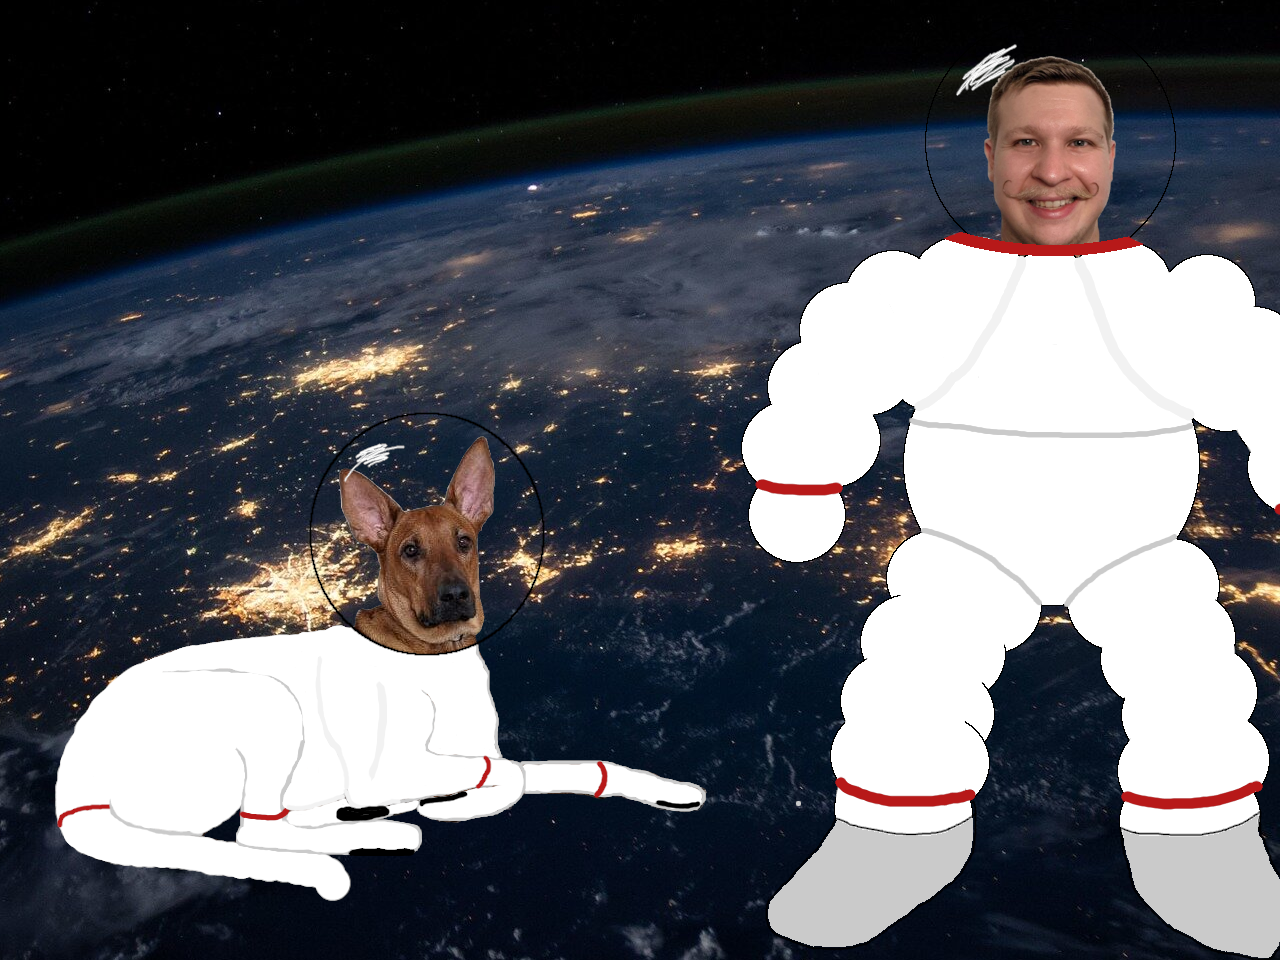
\includegraphics[width=.9\linewidth]{space-dog.png}
\end{center} \cb{F}rankenstein Simon und ich prosten uns 
zu. Auf dem Fernseher zoomt die Kamera langsam auf ein
Raumschiff. Im Inneren des Raumschiffs klingelt ein Wecker. Captain
Simon schreckt auf. Da er in der Schwerelosigkeit des Weltalls war
resultiert seine ruckartige Bewegung darin, das er einen Überschlag
nach dem anderen an Ort und stelle machte.

\begin{center}
"Ah mir wird schlecht! Hundetier, komm her Herrchen braucht dich!"
\end{center}

\noindent Schwanz wedelnd erschien ein Hund im Türrahmen. Anstatt,
wie trainiert zum Schwerkraftschalter zu fliegen steuerte die Hündin
direkt auf den Purzelbaum schlagenden Captain zu. Der
Raumschiffscomputer übersetzte die Hundegedanken in menschlich
verständliche Worte und spielte dies mit einer Computer stimme über
die Lautsprecher ab:

\begin{center}
"Spielen, spielen, spielen!!!! SPIEL MIT MIR!!!"
\end{center}

\begin{center}
"Hundetier, nein! Nicht spielen, du \ldots{} Ah hör auf mich abzulecken
\ldots{} du sollst die Schwerkraft einschalten", brachte Simon lachend
heraus während er sich halbherzig gegen den Hund wehrte.
\end{center}

\noindent Hundetiers Liebesbeweise führten dazu das dass
Hund-Mensch-Purzelbaum-Bündel Richtung Wand trieb. Nach einem Schlag
auf die Schwerkraftschalter saß Captain Simon samt freudig
schwanzwedelndem Hund auf dem Boden.

\begin{center}
"Hundetier, es reicht, sonst muss ich mich ja gar nicht mehr
duschen."
\end{center}

\noindent Das Raumschiff bestand aus einem großen, zylinderförmigen
Rumpf, 4 Solarflügeln, die zur Energie Erzeugung in verschiedene
Postionen gebracht werden konnten, einer Hyperaumantenne an der
Frontseite und 3Photonenexhaust am Ende. Um künstliche Schwerkraft
zu erzeugen, konnte der Zylinderrumpf um eine innere
Versorgungsröhre rotiert werden. Die Petalkraft ermöglichte es auf
der Innenseite des Zylinders zu stehen, wie wenn es ein
Gravitationsfeld gäbe. Simon, schlang die Arme um den Hund, drückte
den Schwerkraftschlater und stieß sich vom Boden ab. Sie segelten,
freudig bellend auf den Zugang zur zentralen Verbindungsröhre. In
der Röhre herrschte zwar Schwerelosigkeit, aber auch ein sanfter
Luftzug, der gesteuert werden konnte um einem der vier Abschnitte
des Raumschiffs zu erreichen.

\begin{center}
"Hey Google\footnote{Ja genau, in dieser Realität gibt es 2021 schon
Hyperraumfahrt - und überall steckt ein bisschen Google\copyright mit
drin. Was denkt ihr wie ruhig die alle schlafen können, wenn 24/7 auf
sie \emph{aufgepasst} wird - \textbf{Anmerkung des Chronisten}}, Abschnitt 1", sagte Simon laut und deutlich.
\end{center}
Der Luftstrom Sog setzte unvermittelt ein und trieben Sie bis zum
vorderen Ende der Röhre und durch eine runde Öffnung ins Innere
des 1. Raumschiffsabschnitt

\begin{center}
"Hey Google, Schwerkraft an", bat der Captain.
\end{center}

Die Außenröhre begann sich langsam zu drehen und Hund und Herrchen
sanken nach unten bzw. wurden nach außen gedrückt. Nach einer
sicheren Landung stand die Raubtierfütterung an. Hundetier schmatze
genüsslich ihre Zorks mit Mürschlam - mit echtem Truthahn Der
Captain absolvierte das all morgendliche Pflichtsportprogramm auf
einem Laufband - die häufigen Phasen der Schwerelosigkeit könnten
sich sonst negativ auf die Muskulatur und Knochendichte auswirken,
und begab sich anschließend unter die Dusche. Anhand dieser
Beschreibung sollte wohl auch klar sein, das eine ganze Menge
Gerätschaften im Abschnitt 1 untergebracht waren. Neben der Dusche,
dem Hundekorb und einem Minigym gab es auch eine kleine Einbauküche
und ein Sofa. Als der Captain frisch und fertig war stand das
morgendliche Briefing, an. Um nicht unnötig Energie zu verschwenden
entschied sich Simon, die künstliche Schwerkraft nicht wieder zu
deaktivieren In jedem Abschnitt gab es eine Leiter, die zur
Verbindungsröhre führte. Bevor er sich in Abschnitt 2, die
Kommandozentrale begab kümmerte er sich noch um den
Hundetierspieltrieb:

\begin{center}
"Hey Google, Aktiviere Roboter a3 und starte \emph{Mit Hund spiel Sequenz
A3Beta7}", wies er den Schiffscomputer an.
\end{center}

\noindent Die Kommandozentrale war deutlich kleiner und
humanonly. Das lag vor allem daran, das ein spielwütiger 4Beiner
gerne mal mit einem aufgeregten Schwanzwedeln den einen oder anderen
Schalter umlegen könnte, wodurch in der Vergangenheit schon der ein
oder andere ungewollte Hyperraumsprung stattgefunden hatte. Simon
ließ sich in einem futuristischen Kommandostuhl nieder und schon
ertönte dass vertraute Geräusch von Spaceskype. Ganz ohne Bildschirm
dafür als leicht, transparentes 3D Hologram leuchtet das Symbol des
Programms in der Luft. Mit einer Geste nahm Simon das Gespräch an und
das Symbol zerfloss und bildete die durchsichtige Darstellung seiner
Supervisorin, die künstliche Lebensform Alpha-beta-iota-tau-chi,
oder wie Simon sie heimlich nannte "A Bitch" - schau dir nochmal
genau den Namen an. Praktischerweise filterten seit 2011 in dieser
Realität alle Computer sämtliche vulgären, sexistischen oder
rassistischen Ausdrücke und wandelte diese in politisch Korrekte
um. Dass ganze war so extrem, dass ein running Gag beim Versenden
von Nachrichten war zu versuchen Sätze so zu bilden, das Software
Bugs dazu führten, das harmlose Sätze mit massiven Grammatik und
Rechtschreibfehlern durch die Korrektur zu Nachrichten von
unangemessener Natur wurden. Ein weiteres Phänomen das
Wissenschaftler feststellten war auch das aufgrund der Tatsache, das
alles und alle permanent zensiert wurden, die Verwendung von
vulgärer, sexistischer und gerade so vor schwarzem Humor triefender
Sprache extrem zugenommen hatte.

\begin{center}
"Hey Bitch, sorry Abitch", begrüßte Simon die AI. Der
Computer sendete \emph{Guten Morgen Alpha-beta-iota-tau-chi}
\end{center}

\begin{center}
Der Computer spielte die Antwort der AI mit einer eigenständigen,
femininen Computerstimme ab: "Guten Morgen Simon. Es ist
0-alpha-omikron-Cola Spacetime. Dein Auftrag lautet an diesem
Spacetag\footnote{Ungefähr eine Woche auf der Erde.} Inspektion von Basis", der Computer wusste das Simon
den 50stelligen Code der Basis nicht wissen wollte und ersetzte
diese daher mit ein von Simon definierten Begriff, "Penis3 auf dem
Asteroid Popel5. Irgendwelche Fragen?"
\end{center}

\begin{center}
"Irgendwelche ungewöhnlichen Vorkommnisse auf Popel5 oder in der
Basis Penis3?", erkundigte sich Simon, gewohnheitsmäßig ohne eine
ernst zunehmende Antwort zu erwarten.
\end{center}

\noindent Die AI hielt inne, während ihr Computerhirn alle, und ich
meine ALLE Daten, die bezüglich der Basis, dem Asteroid und dem
gesamten Quadrant vorlagen, analysierte. Als sie fertig war
antwortete Sie:

\begin{center}
"Keine weiteren Einträge." Die Übertragung wurde beendet.
\end{center}

\begin{center}
"Na klasse, eine Standard, Aussenbasisnspektion - die langweiligste
Aufgabe im Universum", jammerte Simon.
\end{center}

\noindent Nach ein Befehlen an den Computer, begab sich das
Raumschiff auf eine Kurs, der mit der Flugbahn des Asteroiden Popel5
kreuzte. Die Raumschiffe in diesem Universum waren sehr leicht zu
steuern und machten praktisch alles von alleine - manchmal wunderte
sich Simon, wieso es überhaupt menschliche Raumschiffsbesatzungen
gab. Simon deaktivierte die Schwerkraft und begab sich in Abschnitt
3 - die Außenemissionsschleuse Per Computer beorderte er auch seinen
Emotionalsupporthund in den Abschnitt. Simon legte erst dem Hund
seinen Raumanzug an und zog sich dann selbst an. Der
Raumschiffscomputer verkündete die Landung auf Popel5 und nach einer
langwierigen Andockprozedur verließen Simon und Hundetier das
Raumschiff und standen auf der Oberfläche von Popel5. 100Meter
entfernt prankte eine große mechanische Schleuse auf einer
Felswand. Die Basis war in das Innere eines Miniaturgebirges auf Popel5
gebaut. Ohne Schwierigkeiten erreichten die Beiden die Schleuse, die
sich brav öffnete und nach einigen Minuten des Druckausgleichs und
der Dekontamination verließen sie die Schleuse ins innere der
Basis. Das Standardprotokoll der sah für die Inspektion von Basen
vor das der Raumanzug der Begleithunde zuerst, und der des
Raumfahrers erst 30min später geöffnet werden sollte. Für den Fall,
dass die Sensoren einen Fehler gemacht hätten und z.B. eine tödliche
Gasatmosphäre vorherrschte Aber intern hielt sich so gut wie kein
Pilot oder Captain daran. Der Hauptgrund war ganz schlicht Faulheit
und ein blindes Vertrauen in Technologie mit der jeder Mensch seit
den Kleinkindtagen vertraut war. Aber ein bisschen hing es auch
damit zusammen, dass die Vorstellung, den Hund, den einzigen Freund
im Umkugel von 100ten von Lichtjahren zu verlieren eine
schrecklichere Vorstellung als der eigene Tod war. Als Simon die
Hände an den Rand der Helm kuppel legte begann Hundetier wild zu
bellen. Hundetier sprang ihn an, tanzte um ihn herum und wedelte
wild mit den Schwanz.

\begin{center}
"Ja gleich! Ich spiel ja gleich mit dir. Ja was ist den los \ldots{}",
versuchte der Captain seinen Hund zu beschwichtigen. "Jetzt lass
mich doch meinen Helm abnehmen", bat Simon.
\end{center}

\begin{center}
Zeitversetzt, aber Gott sein Dank noch rechtzeitig sprang der
Computer der Basis als Hundegedankenübersetzer ein: "NEIN, HELM AUF!" 
\end{center}

\noindent Alarmiert hielt er inne. Irgendwas stimmte nicht. Dann
erschien ein besorgter Ausdruck auf Simons Gesicht Wo war die Crew?
Ihm war schon klar, das niemand begeistert davon war wenn der
Kantineninspektor zu Besuch kam, aber es war schon sehr komisch das
die Emotionalsupporthunde der Station nicht längst um ihn und
Hundetier herumtanzten. Irgendwas schreckliches war geschehen.

\section{Squidgame}
\label{sec:orgdbfb439}
\begin{center}
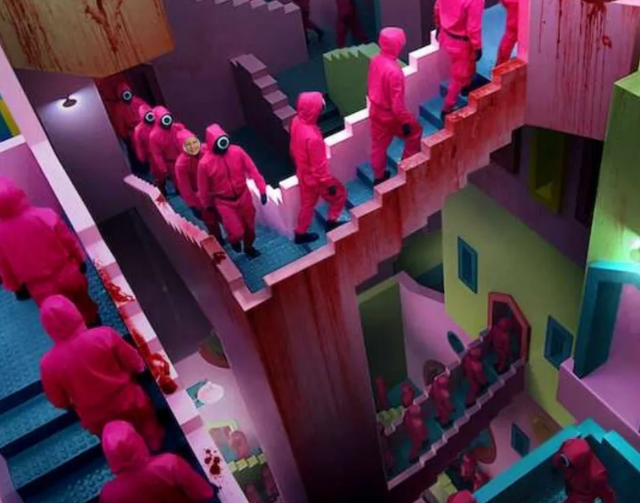
\includegraphics[width=.9\linewidth]{capa-squid-game.png}
\end{center} \cb{Z}app. Frankenstein Simon hatte den
Sender gewechselt. Hey kuck mal in dieser Realität sind wir ein
Steampunkoverlord! Sollen wir uns das angucken? Auf dem Fernseher
erschien ein unrealistisches Luftschiff aus Stahl und Dampf. Dass
Gefährt schob sich langsam über den Bildschirm und unserer Konterfei
breitete sich über die Hülle des Fernsehbildschirms. Die Kamera
zoomt heraus und gab das ganze Luftschiff samt vertrautem Symbol
auf dem Leitwerk zum Vorschein.

\begin{center}
"Na klasse, in dem sind dir Steampunkhitler!", bemerkte Frankenstein
Simon trocken und wechselte den Kanal.
\end{center}

\begin{center}
"Ich hab die Faszination mit Steampunk eh nie so ganz
verstanden. Hast du mal auf die Straße geguckt? Hast du mal gesehen,
wie einer im Winter seinen Diesel startet? Wir leben im
Steampunkzeitalter!", stimmte ich zu.
\end{center}

\begin{center}
"Simon in der Steinzeit \ldots{} Simon in den goldenen 20er \ldots{} oh kuck
Simon als Rabbi von Prag!", kommentierte mein Drinkingbuddy.
\end{center}

\begin{center}
"Hahaha, wie cool der Golem den wir da bauen ist nicht aus Lehm
sondern Leberkas!  Scheint eine Realität mit flexiblen Kosherregeln
zu sein", fiel mir auf.
\end{center}

\noindent Frankenstein zappte weiter will drauf los. Erst tauchte ich
mit einer Perücke, an einem Klavier sitzend auf - Mozart. Dann mit
Perücke auf einem Pferd - alter Fritz. Dann mit Perücke und
E-Gitarre - Bryan May. Zapp. Auf dem Bildschirm erwachte meine
Inkarnation dieser Realität in einem großen Betten-lager Er trug
einen grünen Trainingsanzug mit einer Nummer 11 auf der Brust. Um
ihn herum, erwachten unzählige weitere Männer und Frauen alle in
grünen Trainingsanzügen. Am vorderen Ende des Sporthallen großen
Raums öffnete sich eine Tür und maskierte, rosarot gekleidete
Personen marschierten quietschend ein.

\begin{center}
"Ist nicht dein Ernst! Das ist eine Realität in der es Squidgame
gibt, und wir nehmen daran teil!", rief ich überrascht aus.
\end{center}

\begin{center}
"Now we are talking!", stimmte mir Frankenstein zu.
\end{center}

\noindent \emph{Disclaimer:} Lieber Leser, falls du entweder von der
koreanischen Serie \emph{Squidgame} noch nichts gehört hast, oder noch
nicht fertig damit bist dir diese anzusehen, so sei hiermit gewarnt,
dass diese - wenn auch natürlich tatsächlich so stattgefundene
Geschichte - selbstverständlich Spoiler enthält.

\noindent Alle Personen in der Sporthalle trugen Sportschuhe mit
weißen Sohlen und die Lotto zahlen am kommenden Freitag sind
1-2-3-4-5-6, glaubt mir ganz bestimmt.

\begin{center}
"Tam! Tam Tam Tam! Tam Tam Tam", rief einer der Grünen.
\end{center}

\begin{center}
"Was machst du da?", wollte sein Bettnachbar wissen.
\end{center}

\begin{center}
"Na das ist die ikonische Titelmusik", kam die Antwort.
\end{center}

\begin{center}
"Nein, nein die Geht so: Üüü i \ldots{} Üüüü i \ldots{} Üüü iii", korrigiert
der Fragesteller
\end{center}

\begin{center}
Ein dritter mischte sich ein "Nein, nein, die geht so \ldots{}"
\end{center}

\noindent In diesem Moment bauten sich einige Rosarote bedrohlich
vor den Sängern auf. Die Frage nach der Titelmusik war damit
beendet. Die Rosaroten formten eine Reihe und die Grünen watschelten
bedröppelt auf sie zu. Es waren so um die 50 Personen in grün und 9
Rote. Der mittlerste der Maskierten hob ein Mikrofon zu seinen
Lippen, vergaß allerdings dass er eine Maske trug. Ein lautes
Quietschen ertönte als das Mikro mit Ruck gegen den Maske stieß. Die
Hälfte der Grünen und einige Roten hielt sich instinktiv die Ohren
zu. Irritiert bewegte er das Mikro etwas nach vorne und begann dann
zu sprechen:

\begin{center}
"Liebe Leute, ich hoffe ihr habt alle gut geschlafen."
\end{center}

\begin{center}
"Lauter!", kam es von den billigen Plätzen.
\end{center}

\noindent Der Sprecher bewegte das Mikro instinktive näher zu seinem
Mund - Schrilles Quietschen - Leute rissen ihre Hände zu den
Ohren. "Tschuldigung", murmelte der Rote. Er pfriemeln am Mikro,
bewegte es dann vorsichtig zu seinem Mund und sagte:

\begin{center}
"Es freut uns, dass so viele von euch bereit sich Leib und Leben bei
den alljährlichen Hungergames aufs Spiel zu setzen \ldots{}", einer
seiner Lakaien tippte ihn an, doch er fuhr unbeirrt fort, "Nur einer
von euch wird am Ende überleben, aber diesem Glücklichen erwartet
dann ein Leben voller Luxus."
\end{center}

\noindent Ein angsterfülltes Raunen ging durch die Menge. Ungefragt
rief jemand mit bunten Haaren:

\begin{center}
"Nur eine\_\textsubscript{r}!  Soviel zeit muss sein!"
\end{center}

\begin{center}
"Alter! Die haben uns gerade eröffnet das wir bei fucking Saw sind
und du machst dir sorgen ums Gendern? Dein Ernst?", stieß ihn sein
Nachbar an.
\end{center}

\begin{center}
"Ich bin nicht ein Alter, Kumpel", näselte der Buntschopf.
\end{center}

\begin{center}
"Ich bin nicht dein Kumpel, Buddy", kam die Antwort im Chor von fast
allen Anwesenden.
\end{center}

\noindent Der Sprecher neigte nun endlich seinen Kopf zu dem
Antipper, der ihm hastig einiges zu wisperte Auch ohne ein Gesicht
war klar das er überrascht wenn nicht so gar peinlich berührt
war. Zögerlich drehte er sich wieder zu den Leuten:

\begin{center}
"Okay, mein Fehler das sind hier wohl doch nicht die Spiele um Leben
und Tod, tut mir leid."
\end{center}

\noindent Einer der Männer in grün wurde panisch. Er blickte wild um
sich, tippte dann einen anderen an, "Du bist!", und begann Richtung
Tür zu laufen. Allerdings vergaß er das sich die Türen nach innen
öffneten. Krachend klatschte er dagegen und kippte wie ein Brett
nach hinten um. Der Anführer der Roten gab ein Handzeichen, zwei
maskierte mit roten Kreuzen eilten zum Verletzten. Er drehte sich
zurück zu den Grünen und hielt sich das Mikro vor den Mund - Es
krachte und Quietschte. Einige zuckten reflexartig in eine
Embryonalstellung zusammen.

\begin{center}
"Wisst ihr was? Mir ist das viel zu blöd!", kam es dumpf von der
Maske des Anführers.
\end{center}

\noindent Hastig nahm er besagte ab und strich sich die
verschwitzten Haare aus der Stirn. Ohne ohrenzerreisende Töne begann
er in dass Mikro zu sprechen:

\begin{center}
"Okay, wie mir mein assi - Dave - gerade gesagt hat sind das hier
keine Spiele auf Leben und Tod."
\end{center}

\noindent Aus den Reihen der Adilettenträger war ein einzelnes "Oh
schade!" zu hören.

\begin{center}
"Ja, ja ich weiß was für eine Schande. Aber das Problem ist, das der
Sender, immer gerne eine Fortsetzung haben will. Und es ist relativ
schwierig die beliebtesten Teilnehmer, der letzten Staffel
einzuladen, wenn die alle mausetod sind."
\end{center}

\noindent Ein alter Mann vor Squidgame Simon rief dem Unmaskierten
zu:

\begin{center}
"Ich habe ein Frage!"
\end{center}

\noindent Der Mann nickte ihm auffordernd zu.

\begin{center}
"Ich muss mal"
\end{center}

\begin{center}
"Ja gleich. Sonst noch irgendwelche Fragen?"
\end{center}

\noindent Einige Arme hoben sich. Der erste fragte: "Wo sind die
Klos?"

\begin{center}
"Ja gleeeich! Sonst noch welche Fragen?", wieder gingen Hände hoch,
"Die nichts mit Pipi machen zu tun haben?" Alle Hände gingen nach unten.
\end{center}

\begin{center}
"Na gut, machen wir es nicht spannender als nötig. Liebe Teilnehmer,
ihr seid hier um an den nicht tödlichen und daher auch deutlich
weniger lukrativen Tintenfisch spielen teilzunehmen", erklärte der
Maskenlose in rosarot.
\end{center}

\noindent Dann setzte er einen Jahrmarktsausrufer Gesichtsausdruck
auf rief:

\begin{center}
"Jeder von euch, der es schafft alle 6 Spiele zu gewinnen beeeeeee
\ldots{}. koooooooo \ldots{}. mmmmmmmt \ldots{}"
\end{center}

\noindent Der Lakai tippte ihn erneut an. Genervt drehte sein Chef
sich zu ihm um:

\begin{center}
"Was, Dave!?"
\end{center}

\noindent Der Lakai wisperte ihm Sachen zu während der Boss überrascht Fragen
einstreute:

\begin{center}
"Wie keine 6Spiele? Was meinst du nicht politisch korrekt? Was ist
mit \emph{wer hat Angst vor dem} \ldots{} okay, verstehe. Aber was ist mit \emph{10
kleine} \ldots{} oh \ldots{} oh ja versteh ich jetzt \ldots{} und \ldots{} oje oje"
\end{center}

\noindent Er richtete sich zu den Spielteilnehmern.

\begin{center}
"Okay Jungs, hört mal zu", begann er nur um wieder unterbrochen zu
werden. "Und Mädchen!"
\end{center}

\noindent Zwischen zusammengebissenen Zähnen knurrte er:

\begin{center}
"Buntschopf, sag mir eine Zahl zwischen 1 und 10" Der Angesprochene
erwiderte unsicher:
\end{center}

\begin{center}
"11?"
\end{center}

\begin{center}
"Du bist raus! Und der Rest von Euch spielt jetzt Schafkopfen um das
Preisgeld, ich hab nämlich keine Bock mehr!"
\end{center}
\section{It support - Eine Dragiködie}
\label{sec:orgcea5b73}
\begin{center}

\includegraphics[width=.9\linewidth]{it-support.png}
\end{center} \cb{B}ock auf das Schafkopfturnier? Frankenstein
Simon wartet meine Reaktion gar nicht ab und schaltet direkt
weiter.

\begin{center}
"Hello IT, have you tried to turn IT on and off again?", klang die
Stimme aus dem Telefonhörer. 
\end{center}

\noindent It Support Simon blickte verwirrt aus der Wäsche, dass war
doch sein Text?

\begin{center}
"Hallo hier ist Jörg aus 4. Stock ich habe Probleme mit meinem
Computer", erklärte der Anruf als sich Simon einige Sekunden nicht
gerührt hatte.
\end{center}

\begin{center}
"Hi Jörg, Simon hier, was gibts denn?", erkundigte sich Simon.
\end{center}

\begin{center}
"Naja, mein Computer geht halt nicht, ich hab schon alles
probiert.", behauptete der Vicepresident of Sales aus
dem 4. Stockwerk. 
\end{center}

\noindent Simon massierte sich die Schläfen. Das war das vierte mal
diese Woche, das einer der unzähligen Vicepresidents dieser Firma
angeblich ein unlösbares Problem mit dem Computer hatte. Am Ende war
es immer dasselbe.

\begin{center}
"Okay, Jörg hast du schon mal versucht \ldots{}", begann Simon mit der
Fehleranalyse, doch Jörg unterbrach ihn schnippisch:
\end{center}

\begin{center}
"Den Computer neu zu starten? Ja woohoo wenn ich das nicht schon
versucht hätte, ist das eigentlich das einzige was ihr It Support
Leute könnt? Computer neu starten?"
\end{center}

\noindent Simon ließ die Augen über den linken Bildschirm
schweifen. Er drückte \textbf{F5} um den Browsertab neuzuladen - Stockwerk
4, Arbeitsplatz 32, Jörg Jansen. Ein blaues sleep zeigte das der
Computer entweder aus, oder im Sleepmodus war - ein Druck auf den
Anschalter würde das Problem beheben. Simon könnte den Computer auch
von hier mit einem Klick seiner Maus fern starten Er blickte auf die
Uhr, Zeit für einen Kaffee? Die Kaffeemaschine im 4. war um einiges
besser als die im IT Support Außerdem war Erika die Sekträtin eine
gute Freundin von Simon.

\begin{center}
"Jörg bist du da? Ich schnappe mir mal mein Werkzeug und schau rauf
zu euch. Hoffentlich ist es kein Virus, fass am besten nichts an"
\end{center}

\begin{center}
"Oh Gott oh Gott, beeil dich", dramaqueente Jörg am anderen Ende.
\end{center}

\noindent Der hausinterne IT Support saß im Keller des Gebäudes. Das
war allerdings weniger schlimm wie es sich anhörte, denn 80\% der
Zeit verbrachte man damit den Computer eines Mitarbeiters zu
"reparieren", einen "neuen" Computer auszuliefern oder einen
"kaputten" Computer abzuholen. 10\% der Zeit reparierte man
tatsächlich etwas oder kaufte Ersatz und der Rest ging für
Systemupdates und Pflege drauf und da war es praktisch das die
Server ebenfalls im Keller standen. Simon machte auf seinem Weg halt
im 2. Stock. Er verließ den Aufzug und hatte sofort Frau Kramer an
Hacken wie einen Bluthund. Sie folgte und bombardierte ihn mit Büro
Tratsch während er sich mit eingezogenem Kopf in die Küche stahl. Auf
dem Tisch stand ein Karton mit Donuts. Simon griff sich eine
Pundingbreze und wand sich resigniert zu Frau Kramer.

\begin{center}
"Frau Kramer, wo drückt der digitale Schuh", sagte er ohne jede Hoffnung.
\end{center}

\begin{center}
"Oh ja, wenn Sie schon mal da sind, mein Computer macht so komische
Dinge", erwiderte die Frau.
\end{center}

\begin{center}
"Erzählt er Ihnen Witze, oder was?", rutsche es ihm heraus.
\end{center}

\noindent Frankenstein Simon und Ich prosteten uns belustigt zu. Frau
Kramer bemerkte den Sarkasmus in seiner Stimme nicht und erklärte
fröhlich:

\begin{center}
"Nein nein, sehen Sie da sind so komische, so Fenster?"
\end{center}

\noindent Stirn runzelnd überlegte Simon ob er sie darauf hinweisen
sollte, dass der Name \emph{Windows} nicht von ungefähr kam, verkniff es
sich dann aber. Er ging zu einem der Hängeschränke, nahm einen
Teller heraus und legte das Gebäck darauf. Dann nahm er noch einen
Donut, legte diesen auch auf den Teller. In der Einbauküche wusch er
sich die Hände, nahm seinen Teller und wies mit der Hand Richtung
Tür.

\begin{center}
"Na gut, schauen wir uns das doch mal an Frau Kramer"
\end{center}

\noindent Simon setzte sich auf den noch warmen Bürostuhl und tippte
eine beliebige Taste um den Computer aufzuwecken. Dann probierte er
dass Passwort, das Frau Kramer seit Jahren nicht geändert hatte
aus. Er hatte schon versucht es zu ändern, bzw. mit ihr für sie es
zu ändern, aber die folgenden 2Wochen hatte sie das neue Passwort
42 mal vergessen - und so gut waren die Donuts im 2. nun auch wieder
nicht. Daher hatte er den Computer von Frau Kramer im Haus komplett
geblacklistet - von diesem Computer konnte man nun auf gar nichts
hausintern relevantes mehr zugreifen. Erstaunlicherweise konnte Frau
Kramer ganz normal weiterarbeiten.

\noindent Die Kinder von Frau Kramer und ein flache graue Leiste am
unteren Bildschirmrand lachten Simon ins Gesicht. Er drehte sich zur
wie ein Honigkuchenpferde essenden und grinsend Frau. Dann stellte
er die 2. häufigste Frage in seinem Berufsalltag:

\begin{center}
"Wie lange ist das letzte Update her?"
\end{center}

\noindent Windows95 sah komisch aus auf dem großen
Bildschirm. Augenblicke später erschien ein Popup, dann noch
eines. "Kaufen Sie Penispumpen!" "Dieser Trick wird Sie
überraschen!"

\begin{center}
"Sehen Sie? Diese Nachrichten meine ich", rief Frau Kramer erfreut.
\end{center}

\begin{center}
"Ich habs mir fast gedacht", antwortete Simon kopfschüttelnd.
\end{center}

\noindent Der IT-Supportler warf einen Blick unter den Tisch. Hm
Pentium2 \ldots{}

\begin{center}
"Frau Kramer, Sie haben in der Lotterie gewonnen, ich bring ihnen
nachher ein neuen Rechner - und dieses Museumsstück wandert in den
Müll."
\end{center}

\begin{center}
Besorgt fragte sie schnell: "Aber schon wieder mit meinem Passwort, ja?"
\end{center}

\begin{center}
Simon kratzte sich an der Nasenwurzel. "Ja, mit ihrem Passwort, ich
richte es gleich ein"
\end{center}

\noindent Der nächste Zwischenstopp war im 3. Hier hausten etwas mehr
tech savvy Mitarbeiter. Simon klopfte an einer Bürotür und trat
direkt ein. Ein Nerd mit Brillengläsern so dick wie Backsteinen
blickte ihn an. Dann starrte er auf Simons Donut.

\begin{center}
"Mach dir keine Hoffnungen, ich hab das Bitte-nicht-Füttern-Schild
gesehen", zerstörte Simon all Träume des Nerds. "Ich hab einen
Code-Zucker, schick mir ne Mail was du haben willst"
\end{center}

\noindent Das Nerdgesicht verzog sich freudig erregt. Ohne weitere
Erklärung verließ er das Büro und ging zurück zum Aufzug. Ein
Code-Zucker war wenn ein Mitarbeiter aus dem 2. Stock einen neuen
Computer braucht. Für Mitarbeiter aus dem 2. Stock gab es praktisch
keinerlei finanziellen Rahmen was die Anschaffung von Büroequipment
anging. Der Grund war, das eine Mitarbeiterin des 2. und Chef der
Firma sagen wir mal eng befreundet waren. Und als die junge Dame
ihrem Freund klar gemacht hatte, dass sie einen schöneren Stuhl, ein
größeres Büro und ein 5000Euro Macbook haben wollte begann der eine
oder andere zu tuscheln. Bzw. als sie das Zeug dann tatsächlich
bekam. Um Gerüchte und Unruhen zu vermeiden kam die Chefin der HR
auf die Idee allen Mitarbeitern im 2. bei Gelegenheit ein paar
Wünsche zu erfüllen - siehe Donuts. Wann immer ein aufgeblasener
2.Stockmitarbeiter nun auf die glorreiche Idee kam einen neuen
Computer zu brauchen begab sich Simon direkt in den 3. Stock wo die
hausinternen Entwickler und Programmierer saßen. Dann trugen sie das
Zubehör eines Dev in den 2., verklickerten dem Computeranalphabeten
es sei der neuste, geilste Scheiß und bestellte dann für den
Entwickler das neuste vom neuen. Und Simon hatte bei praktisch allen
im 3. einen Stein im Brett. Der Fahrstuhl kam zum stehen. Auf dem
Weg zur Kaffeemaschine lief ihm Jörg entgegen.

\begin{center}
"Was dauert das denn immer so lange? Manche Leute müssen auch
arbeiten!", beschwerte er sich direkt, ohne Hallo und Armen. 
\end{center}

\noindent Simon zeigte auf den Donut, dann auf Jörg. Und ging an ihm
vorbei in Küche. Jörg hatte sich augenblicklich einen anderen Ton
angewöhnt. Bei einer Tasse schwarzem Gold tauschten Sie sich etwas
aus. Frankenstein Simon erhob sich aus seinem Sessel und fragte
mich:

\begin{center}
"Auch schwarz, oder?"
\end{center}

\noindent Kurz darauf kam er mit zwei Tassen Kaffee zurück. Der Simon
auf dem Fernsehbildschirm war gerade fertig mit seiner Tasse und dem
Gebäck. Er wusch sich erneut die Hände. Dann gingen er und Jörg zu
dessen Büro.

\begin{center}
"Okay Jörg, dann zeig mir mal was nicht geht", bat er.
\end{center}

\begin{center}
Schon wieder etwas empört setze sich Jörg demonstrativ hin und
begann wild zu tippen und mit der Maus zu klicken. "Da! Siehst du?
Und jetzt sag nicht ich soll ihn neu starten, das Licht leuchtet, er
ist an!", jammerte Jörg.
\end{center}

\begin{center}
"Dann war der Computer vorher scheinbar nicht aus sondern nur im
Schlafmodus gewesen", überlegte Simon, aber ein Blick auf den
schwarzen Bildschirm bestätigte seine 2 Vermutung.
\end{center}

\noindent Simon schaltete Jörgs Bildschirm ein und verließ das Büro
wortlos.

\section{Dr Dolittle}
\label{sec:org73b9943}
\begin{center}
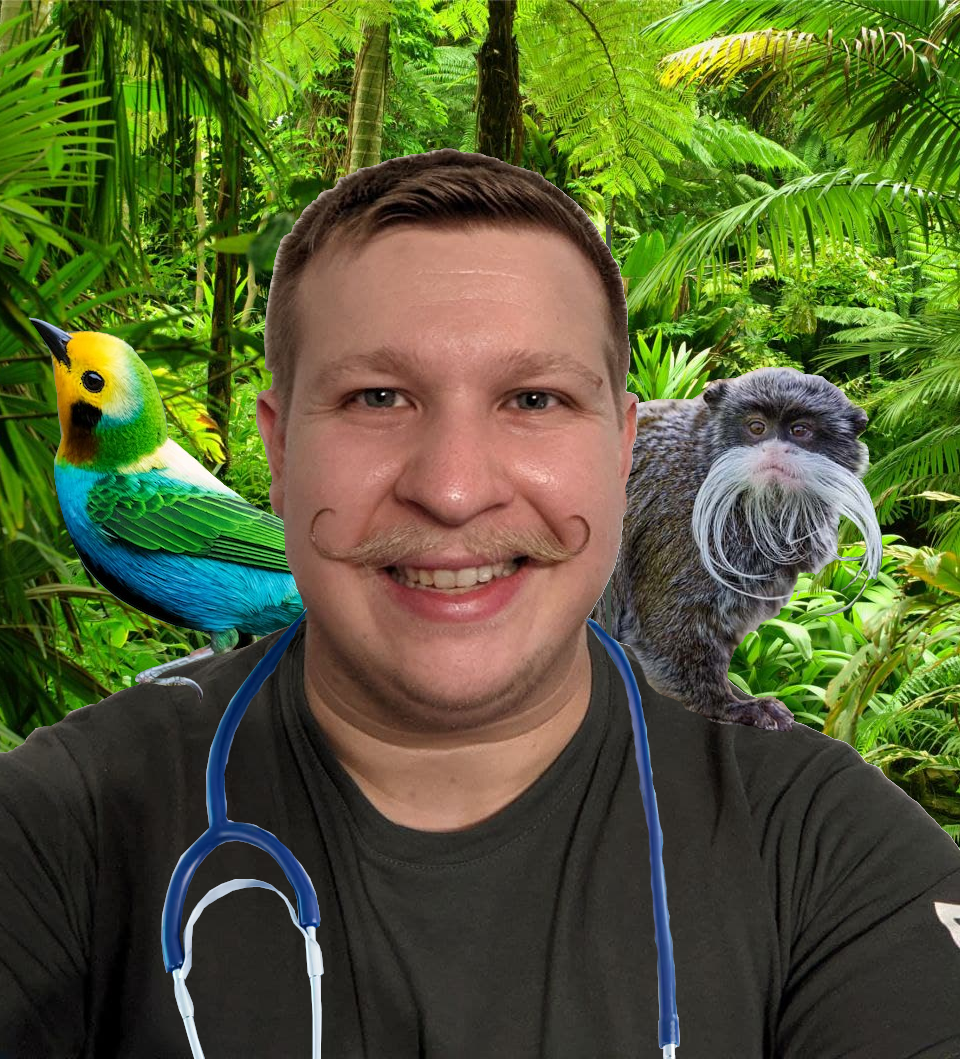
\includegraphics[width=.9\linewidth]{dr_dolittle.png}
\end{center} \cb{H}err Doktor werde ich jemals wieder Geige
spielen können? Die Frage erfüllte den tropisch feuchten Raum im
Baumhaus Sekunden lang mit Atem ergreifender Bedrohlichkeit. Doktor
Simon Dolittle rollte mit den Augen und seufzte schließlich:

\begin{center}
"Nein Jeff, aber das liegt daran, dass du noch nie Geigen spielen
konntest - du bist ein Orang-Utan"
\end{center}

\noindent Jeff, der Orang-Utan kratzte sich nachdenklich am Kopf,
teils um sich daran zu erinnern, ob das stimmte, teils um sich daran
zu erinnern was er gerade gefragt hatte. Doktor Faul fügte nun in
einem etwas empathischerem Ton hinzu:

\begin{center}
"Aber was deine Vergesslichkeit angeht, das Problem werden wir bald
vergessen haben."
\end{center}

\noindent Der Arzt half dem rothaarigen Patienten aus dem
improvisierten Behandlungsstuhl und begleitete ihn zur \emph{Tür}. In
Wirklichkeit war es keine Tür, sondern lediglich ein Loch in einer
Wand des Baumhauses, aber die Patienten hatten in der Regel
keine Probleme die Praxis entweder fliegend oder per Trazangeheul
und Liane zu verlassen. Jeff, bestätigte als Ausnahme die Regel,
indem der vergessliche Affe, zwar die ersten 2Schritte -
raus springen und heulen hinbekam, aber aufgrund seiner
Gedächtnislücken vergaß eine Liane zu greifen. Sekunden später
landete er Kopf voraus auf dem Waldboden.

\begin{center}
"Und ich wunder mich woher die Amnesie kommt?", murmelte Simon mehr
zu sich selbst.
\end{center}

\noindent Aber sein getreuer Assistent Momo das Kaiserbartäffchen
kommentierte gehässig:

\begin{center}
"Leichte Schläge auf den Hinterkopf, fördern das Denkvermögen."
\end{center}

\noindent Jeff rappelte sich wie auf und trottet von dannen. Als der
rote Affe die Szene verlassen hatte öffneten sich die Bäume erneut
für rote Gestalten Genau gesagt eine Reihe von Soldaten in den
Roten Röcken der Britischen Streitkräfte. Zwei trugen absurd lange
Trompeten und verkündeten ihr Eintreffen. Nach den Trompetern und
Soldaten kam nun auch ein älterer Mann mit Perücke ins Bild. Simon
kommentierte die Situation:

\begin{center}
"Na toll, der Gesandte der Königin! Momo, hol Jeff zurück, wir
machen eine kleine Reise nach London"
\end{center}

\noindent Ich blickte zu Frankenstein.

\begin{center}
"Können wir vorspulen? Ich hab irgendwie keinen Bock mir da jetzt
eine mehrwöchige Schiffsreise anzugucken", fragte ich ihn.
\end{center}

\begin{center}
"Wie stellst du dir das vor? Das ist kein Film, das ist die
Realität. Ja okay nicht diese Realität, aber eine Realität und die
läuft jetzt gerade ab, in Echtzeit. Da kann man nicht einfach
vorspringen", gab der verwundert zurück. "Soll ich um schalten?",
erkundigte er sich dann.
\end{center}

\begin{center}
"Ja schalt um. Aber irgendwie würde ich gerne wissen was mit dem
Affen passiert, ich hab da so eine Vermutung", antwortete ich.
\end{center}

\begin{center}
"Wir können ja in den Teletext gucken was passiert", sagte
Frankenstein Simon schulter zuckend "Blahblahblah \ldots{} kurzsichtige
Königin verknallt in Dolittle \ldots{} blablablah \ldots{} heiratet
vergesslichen Affen \ldots{} klingt wie eine ganz normale Ehe", lass
Frankenstein vor.
\end{center}

\begin{center}
"Ich wusste es!", stieß ich hervor.
\end{center}

\begin{center}
"Ja, war irgendwo offensichtlich"
\end{center}

\section{Böser Zwillingsbruder}
\label{sec:orga1db006}
\begin{center}

\includegraphics[width=.9\linewidth]{Simon_with_smoking.png}
\end{center}
\cb{P}inkelpause! Frankenstein erhob sich aus dem Sessel und drückte
auf die Pause taste Das Bild vor uns fror ein - irgendwie hatte ich
die Regeln noch nicht so ganz verstanden. In dem Moment gingen alle
Lichter im Raum an. Sie wurden immer heller, ein hohes elektrisches
Surren und Wumps! Alles war dunkel. Frankenstein schien nicht
überrascht eher genervt. Mich traf es jedoch völlig
unvorbereitet. Was war hier los?

\begin{center}
"Hör auf mit der Show und komm raus", knurrte Frankenstein.
\end{center}

\begin{center}
"Ist das dein Monster?", wollte ich verängstigt wissen.
\end{center}

\begin{center}
"Schön wäre es ja, dann hätten wir wieder Bier! Nein, das ist
Bimon - der böse Simon", erklärte Frankenstein genervt.
\end{center}

\noindent Ein Scheinwerferspot aus dem Nichts erhellte eine Stelle
vor uns. Mit Zylinder, Monokel und Pfeife stand er da - Bimon mein
böser Zwilling. Jede Realität hat neben einem Simon, der meistens
coole Dinge tut, wie im It Support zu arbeiten oder
Weihnachtsgeschichten zu schreiben auch einen Bimon, der naja böse
ist.

\begin{center}
"Ich bin der böse Bimon, und ich bin an allen, ja ALLEN, schlimmen
Dingen schuld die so passieren!", verkündete er unheilvoll.
\end{center}

\begin{center}
"Dann bist du also Schuld, an \ldots{} also an allem? Krieg, Hunger
Armut?", wollte Frankenstein Simon wissen. 
\end{center}

\begin{center}
"Ja!", bestätigte Bimon böse grinsend.
\end{center}

\begin{center}
"An allem Schlimmen was so passiert? Auch daran das ich von Bier
immer so oft zum Pinkeln muss?", wollte ich nun wissen. Bimon
kicherte zufrieden.
\end{center}

\begin{center}
"Und dass an der Tankstelle nie so ein Plastikhandschuh fürs
Dieseltanken mehr ist?", fügte Frankenstein Simon hinzu. Bimon
nickte mit leuchtenden Augen.
\end{center}

\begin{center}
"Das der Parkplatz vor meinem Haus immer weg ist?", fiel es mir wie
Schuppen von den Augen.
\end{center}

\begin{center}
"Besonders das der Parkplatz vor deinem Haus!", krähte Bimon.
\end{center}

\begin{center}
"Das die Besatzung von der Raumstation in der vorherigen Geschichte
verschwunden ist?", fragte Frankenstein.
\end{center}

\begin{center}
"Ja, äh nein, daran bin ich nicht Schuld", wies Bimon die Schuld von sich.
\end{center}

\begin{center}
"Weiß du was mit denen passiert ist?", erkundigte ich mich nun.
\end{center}

\begin{center}
"Spacecovid", antwortete er lapidar.
\end{center}

\begin{center}
"Aber sonst bist an allem schlimmen Schuld?", versuchte ich das
Gespräch wieder in seine Bahn zu lenken.
\end{center}

\begin{center}
"Oh ja", gestand Bimon.
\end{center}

\begin{center}
"Dann bist du sozusagen sowas wie der Teufel?", wollte ich nun von
meinem bösen Doppelgänger wissen.
\end{center}

\begin{center}
"Der Teufel? Was macht der schon schlimmes? Läuft überall herum und
bietet Leute ein IPhone\copyright für ihre Seele an. Wenn ich die
Wahl hätte würde ich das Handy nehmen, wofür ist eine Seele denn
gut?"
\end{center}

\noindent Begleitet von einem Geruch nach Pech und Schwefel öffnete
sich die Fahrstuhltür und ein gehörnter Hüne mit Pferdefuß und
IPhone in der Hand trat heraus.

\begin{center}
"War nur so ein Spruch", sagte der böse Bimon.
\end{center}

\begin{center}
"Och menno", beschwerte sich Satanas und stieg wieder in den Aufzug.
\end{center}

\begin{center}
"An Krebs bist du dann auch Schuld?", erkundigte sich Frankenstein
Simon.
\end{center}

\begin{center}
"Ja, ja und nochmal ja. Ich denke wir können mit dieser Befragung
langsam aufhören. Ich bin böse, das sollte hiermit klar für alle
Leser sein", sagte Bimon scharf.
\end{center}

\begin{center}
"Okay, wie läuft das jetzt ab? Bringst du uns um oder steckst uns
mit Spacecovid an oder was? Für einen angeblich so bösen Bösewicht
machst du relativ wenig böse Dinge", brachte ich zum Bedenken.
\end{center}

\begin{center}
"Ja genau. Naja vielleicht will er auch uns kein IPhone gegen seine
Seele abkaufen - du Arschloch", sagte Frankenstein mit einem Blick
auf den Fahrstuhl. Die Türen waren wieder aufgegangen. Santa kauerte
in der Ecke in Embryonalstellung und weinte. Die Feuerlöschanlage
benetze den Boden der Kabine mit Wasser.
\end{center}

\begin{center}
"Hahaha, eure Beschimpfungen sind wie Lob für mich. Und jetzt werde
ich euch das Hdmi Kabel wegnehmen damit ihr nicht mehr weiter
Fernsehen könnt hahahahah", rief der böse Bimon.
\end{center}

\noindent Er sprang vor, riss das Kabel aus dem Laptop und denn
Fernseher um, fiel hin, sprang auf die Füße, richte sein Krönchen
und rannte auf das Turmfenster zu. Kopf voran tauchte er durch das
Turmfenster und verschwand in der Nacht.

\begin{center}
"Na Klasse, und ich wollte jetzt langsam mit den
Weihnachtsmannthemed Realitäten anfangen! Ach was solls, das wars
wohl dieses Jahr mit den Geschichten", schloss Frankenstein ab.
\end{center}

\noindent Die Fahrstuhltüren gingen auf und ein grünhäutiger Simon
mit Schrauben am Hals kam mit einem Kasten Bier herein.
\section{Outtakes}
\label{sec:org341a73a}
\subsection{Im Leipziger Zoo}
\label{sec:orgecf4171}
\begin{center}
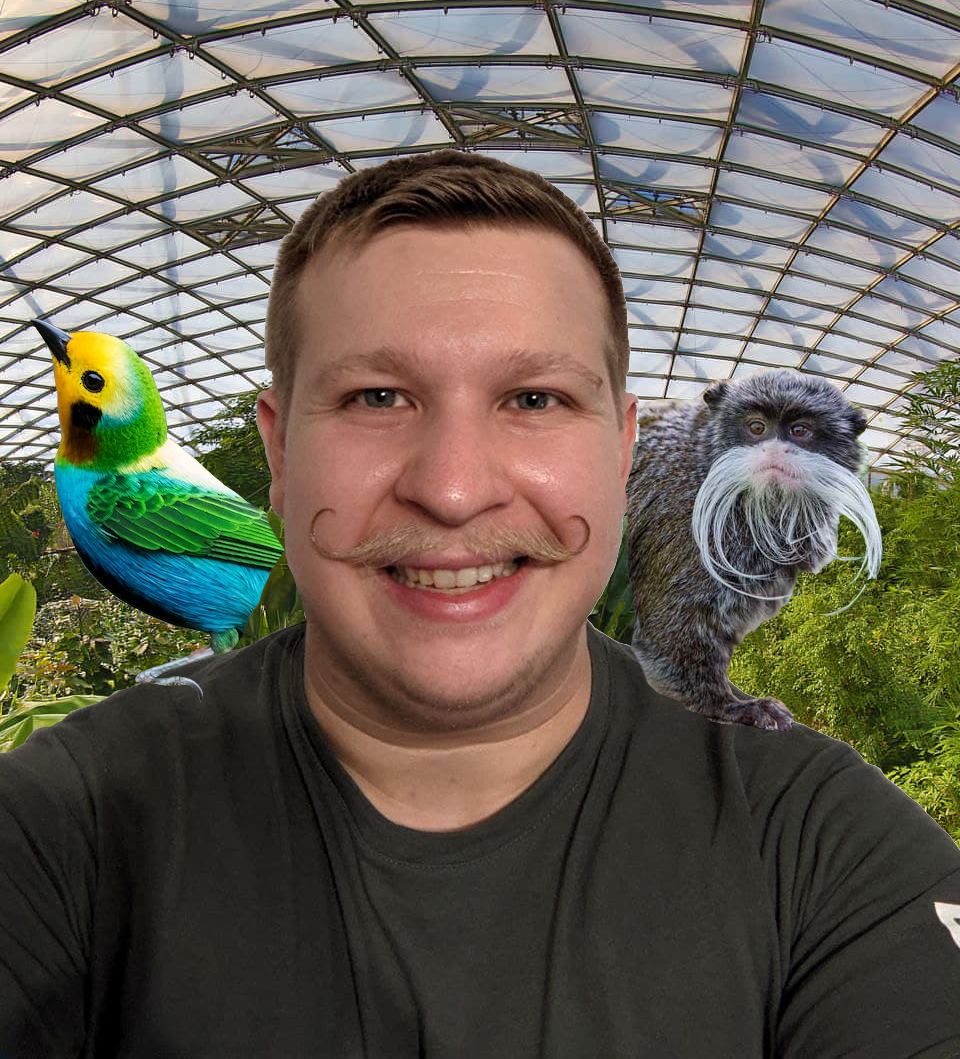
\includegraphics[width=10cm]{figures/leipzig.png}
\end{center}
\cb{A}aaaaaaah! Ein Kind kommt an mir vorbei gerannt. Es ist ein
feucht trüber Tag im Leipziger Zoo. Eigentlich das perfekte Wetter
würde man meinen - wer geht schon bei so einem Wetter in den
Zoo. Aber leider sind die anderen Besucher genauso wettergegerbt
wie meiner einer. Der erste Schreck war, als das Gehege der
Kaiserbartäffchen leer war - wahrscheinlich sind die süßen Racker
schon in einem Innengehege, immerhing winter is coming. Deswegen
hab ich einen solchen Affen auf dem Bild auf meine Schulter
gesetzt, damit ihr wisst wie die aussehen. Sehr coole kleine
Affen. Das Kind rast gerade lachend an mir vorbei, da denke ich mir
noch: "Uh, ist schon gefährlich bei dem feuchten Laub und Pfützen
so zu rennen" und wumms ist es schon passiert. Der Junge
strauchelt, stolpert und macht einen purzelbaum durch mehre
Wasserlachen. Ich stehe ungefähr in der Mitte zwischen dem
heulenden Knirps und den Eltern, oder Tante und Onkel. "Muss ich da
jetzt helfen", überlege ich kurz. Aber bevor ich überhaupt was
machen kann ruft der Vater/Onkel/Opa von hinten:

\begin{center}
"Steh auf! Und hör auf zu heulen!"
\end{center}

\noindent Sichtbar genervt schreitet der Mann, schwer atmend an mir
vorbei. Fast zur Erklärung murmelt er:

\begin{center}
"Das ist das dritte Paar Hosen\ldots{}"
\end{center}

\begin{center}
"Na gut, das sie so viele Ersatzkleidung dabei haben", meine ich.
\end{center}

\begin{center}
"Sie machen sich ja keine Vorstellungen", seufzt er traurig.
\end{center}
\subsection{Ein Kaffeekränzchen in der Hölle}
\label{sec:org9f747cd}
\begin{center}

\includegraphics[width=10cm]{figures/hölle.png}
\end{center}
\cb{I}ch will nicht! I dont care. Weihnachten ist die Zeit im Jahr
in der man Dinge tut, die man am liebsten nicht tun müsste.

\begin{center}
"In 4kilometern nehmen Sie die erste Ausfahrt im Kreisverkehr",
verkündete das Navigationssystem.
\end{center}

\noindent Weihnachten ist auch die Zeit an der, der eine oder
andere sehr einsam ist. Nicht jeder hat eine liebende Familie,
Freunde oder viel Geld um sich glaubhafte Lügner zu kaufen. Seit
ich vor ein paar Jahren, nachzulesen in einer früheren
Weihnachtsgeschichte, dem Teufel über den Weg gelaufen bin, gehört
es zu meiner alljährlichen Festtagsroutine im Land des Feuer und
Schmerz vorbei zu schauen und dem großen Roten ein \emph{Geschenk} zu
bringen.

\begin{center}
"Ich weiß immer noch nicht was ich hier soll", beschwerte sich mein Beifahrer.
\end{center}

\noindent Zu meiner Rechten saß ein hoher Unionspolitiker. Mit
einem Seitenblick und einer sinisteren Ton antwortete ich:

\begin{center}
"Das wirst du schon sehen \ldots{} \emph{Freund} \ldots{}"
\end{center}
\subsection{Das Diner am Ende des Paralleluniversums}
\label{sec:orge2e537b}
\begin{center}
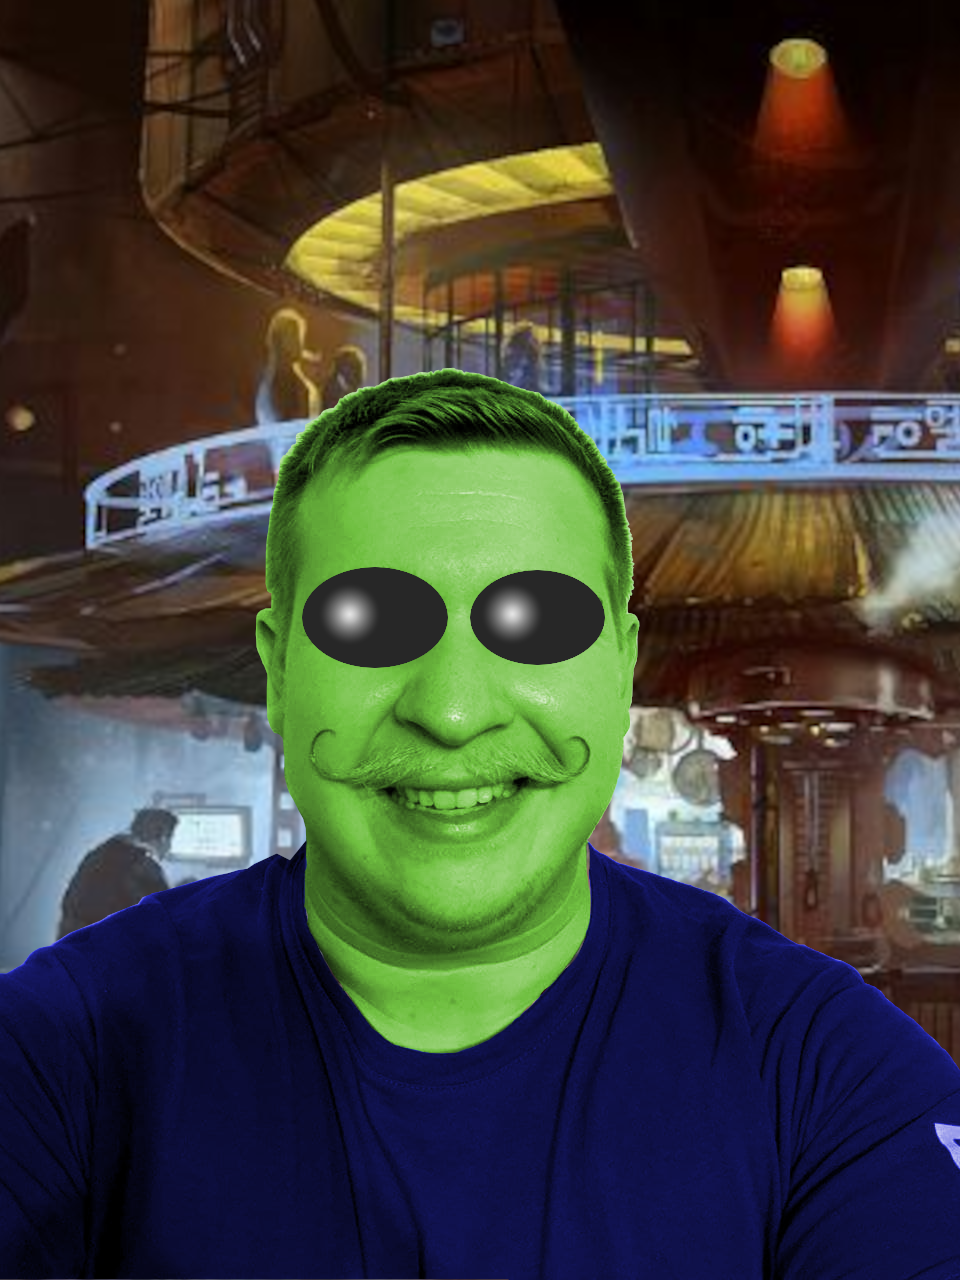
\includegraphics[width=10cm]{alien.png}
\end{center}
\cb{E}inmal Zorks mit Mürschlamp! Ein blaues Alien mit drei im
Gesicht und insgesamt 5Rüsseln rief meine Bestellung aus. Meines
Zeichens Alien Simon leckte ich mir meine Lippen vor
Vorfreude. Zorks mit Mürschlamp ist ein all-time-classic der
intergalaktischen Küche. Das Gericht nimmt nämlich immer die Form
des Gerichts an, das der Essende am liebsten gerade essen
würde. Zum Beispiel Pizza oder Vanille Eis oder das noch pumpende
Herz deines Feindes. In meinem Fall gab es Weltraumspaghetti. Das
tolle an diesen im gegensatz zu herkömmlichen Spaghetti war, dass
sie sich bei hintehaltener Gabel, selbstständig aufwickelten, mit
Soße tränkten und beim Essen nie kläckerten. Ich wollte gerade die
perfekt drapierte Gabel genüsslich zum Mund führen als

\begin{center}
"Alarm! Alarm!", brüllten alle Lautsprecher.
\end{center}

\noindent Verunsicherte drehten ihre zwei bis drei Köpfe
hilfesuchend in alle Richtungen. Ich ließ meine Gabel fallen, griff
meinen Helm und lief hungrig los. Auf meinem Weg zum Hangar holte
mich eine gelbe Gestallt mit langen Haaren ein - Mein Kanonier
Ibes. Ich nickte ihm wortlos zu er keuchte:

\begin{center}
"Weltraumkrake!"
\end{center}

\noindent Verdammte Weltraumkraken! Andere Piloten liefen vor und
hinter uns. Eine große Tür öffnete sich vor uns - der
Spacekampfjethangar. Wir verloren keine Zeit für einen
Preflightcheck und kletterten direkt in unseren Spacefighter. Ich
begann direkt die Startsequenz, schloss die Kanzel und setzte erst
als wir automatisch zur Schleuse schwebten meinen Helm auf.

\begin{center}
"Bereit!", fragte ich im Commsystem.
\end{center}

\noindent Mein Kanonier saß in einer separaten Kanzel hinter
mir. Ich hörte in diesem Moment das Zischen als sich Ibes Kanzel
versiegelt. Das rote Warnleuchten "Kanzel offen" erlosch. Die
Spacekanonen rotierten leer durch als der Kanonier die Waffen auf
Temperatur brachte.

\begin{center}
"Ja, ja sorry, war ne lange Nacht. Okay Ich bin ready, lass uns
Kalamari aus dem Vieh machen!", antwortete er schließlich. 
\end{center}

\noindent Die Schleuse schloss sich hinter uns, und ich gab vollen
Schub. Vor uns türmte sich der größste Spacekraken auf, den ich je
gesehen hatte\ldots{}
\section{Nachwort}
\label{sec:orgd205606}
\begin{center}

\includegraphics[width=.9\linewidth]{taucher.png}
\end{center} \cb{L}iebe Leute, das wars schon wieder von mir für
dieses Jahr. Leider hat der böse Bimon zugeschlagen sonst wären wohl
noch ein paar mehr verrückte Dinge passiert. Gewöhnlich ende ich mit
dem Wunsch das ihr alle Schöne Weihnachten und eine guten Rutsch ins
neue Jahr habt. Und ja auch dieses mal wünsche ich mir das für
euch. Aber viel wichtiger diese Jahr wünsche ich mir für alle von
euch 10000Euro in cash und einen Tauchtrip auf den Malediven. Oh
Scheiß so ein Drecksjahr, da kann man sich doch echt nur besaufen
oder?  Okay der Sommer war ganz gut, und vorlauter geschlossenen
Bars und Abstandregeln hat man am Ende vom Monat doch Tatsachen noch
Geld auf dem Konto aber ist es das Wert? Also lasst uns alle zum
Himmel aufblicken, ein Flugzeug mit einer Sternschnuppe verwechseln
und gemeinsam wünschen: "10000Euro in cash und ein
Tauchurlaub. 10000Euro in cash und ein Tauchurlaub \ldots{}"

\begin{center}
In diesem Sinne fröhliche Weihnachten und einen guten Rutsch ins
neue Jahr, dein Simon.
\end{center}
\end{document}